\documentclass[mathserif]{beamer}
\usetheme{Luebeck}
\usepackage[francais]{babel}
\usepackage[utf8]{inputenc} % Uses the utf8 input encoding
\usepackage[T1]{fontenc} % Use 8-bit encoding that has 256 glyphs

\usepackage[nomath]{kpfonts}
\usepackage{eulervm}
\usepackage{amssymb}
%\usepackage{default}

\usepackage{amsthm}
\usepackage{amssymb}
\usepackage{xparse}
\usepackage{thmtools}
\usepackage{stackrel}

%shortcuts
\newcommand{\R}{\mathbb{R}}
\newcommand{\C}{\mathbb{C}}
\newcommand{\Z}{\mathbb{Z}}
\newcommand{\N}{\mathbb{N}}
\newcommand{\fii}{\varphi}
\newcommand{\dd}{\mathrm{d}}
\newcommand{\CP}{\mathbb{CP}}
\renewcommand{\S}{\mathbb{S}}
\DeclareMathOperator{\Sp}{Sp}
\DeclareMathOperator{\tr}{tr}
\DeclareMathOperator{\dist}{dist}

% theorems configuration

\makeatletter
\newtheoremstyle{indented}
{7pt} %vertical space before
{7pt} % vertical space after
{} %{\addtolength{\@totalleftmargin}{2.5em}
	%\addtolength{\linewidth}{-3.5em}
	%\parshape 1 3.5em \linewidth} %body font
{1.5em} %indent
{\bfseries} %header font
{.} %punctuation
{.5em} %horizontal space after header
{} %header specification

\theoremstyle{definition}

\newtheorem{defn}{Définition}[section]

\theoremstyle{plain}
%\newtheorem*{theorem*}{Theorem}

\newtheorem{thm}{Théorème}

\renewcommand{\thetheorem}{\Alph{theorem}}
\newenvironment{preuve}{
	\noindent \textbf{Proof. }}{\hfill $\square$\medskip\par}

\newtheorem{exemple}[defn]{Example}
\newtheorem{prop}[defn]{Proposition}
\newtheorem{corr}[defn]{Corollary}
\newtheorem{por}[defn]{Porisme}
\newtheorem{ex}[defn]{Example}
\newtheorem{lem}[defn]{Lemma}
\newtheorem{conj}{Conjecture}
\newtheorem{ax}{Axiom}  %Axioms have their own numerotation

\theoremstyle{definition}
\newtheorem{rem}[defn]{Remark} %remarks are not indented
\newtheorem{rems}[defn]{Remarks}

%--------------
% Mise en page mathématique
%--------------
\addtolength{\jot}{.2em}


\title{Spectre à basse énergie des opérateurs de Toeplitz}
\author[Alix Deleporte]{Alix Deleporte\\Sous la direction de Nalini Anantharaman}
\institute[IRMA]{Institut de Recherche Mathématique Avancée}

\AtBeginSection
{
	\begin{frame}
		\frametitle{Plan}
		\tableofcontents[currentsection]
	\end{frame}
	
}

\newcommand{\spline}{\hline}
\renewcommand{\arraystretch}{1.3}
\begin{document}
\begin{frame}
	\titlepage
      \end{frame}

      \begin{frame}
        \frametitle{Introduction}
        \begin{center}
          \only<1>{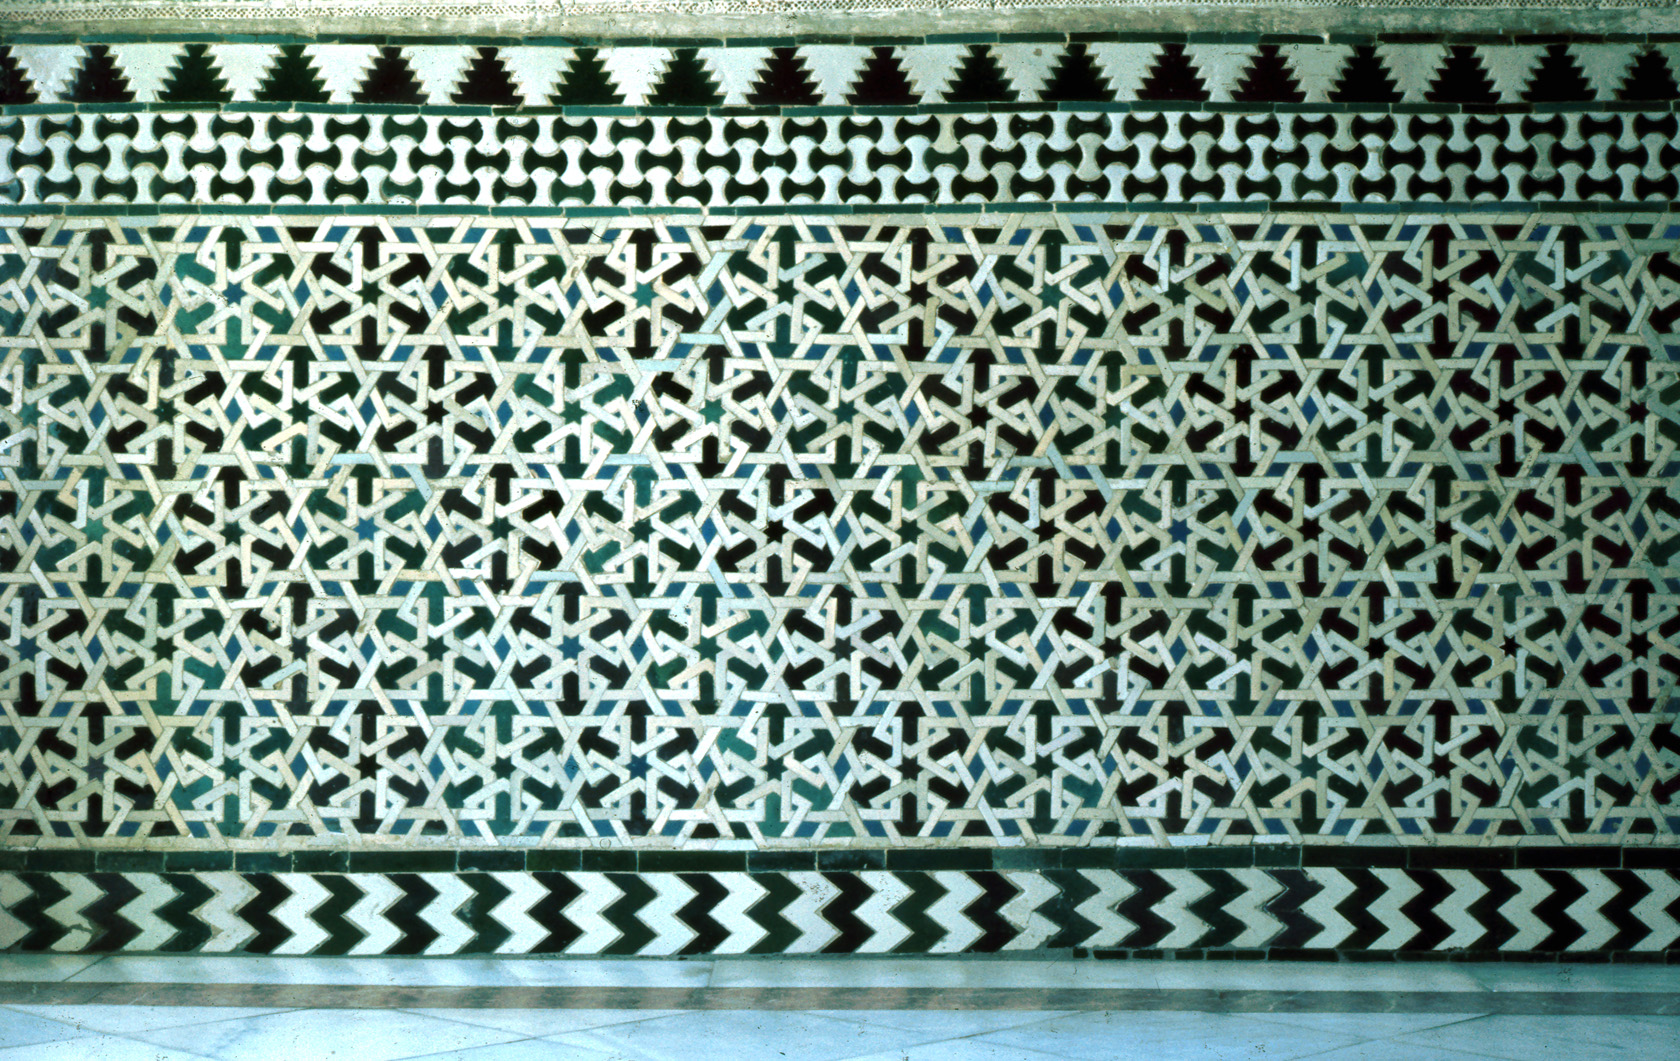
\includegraphics[scale=8]{Alcazar.jpg}}
          \only<2>{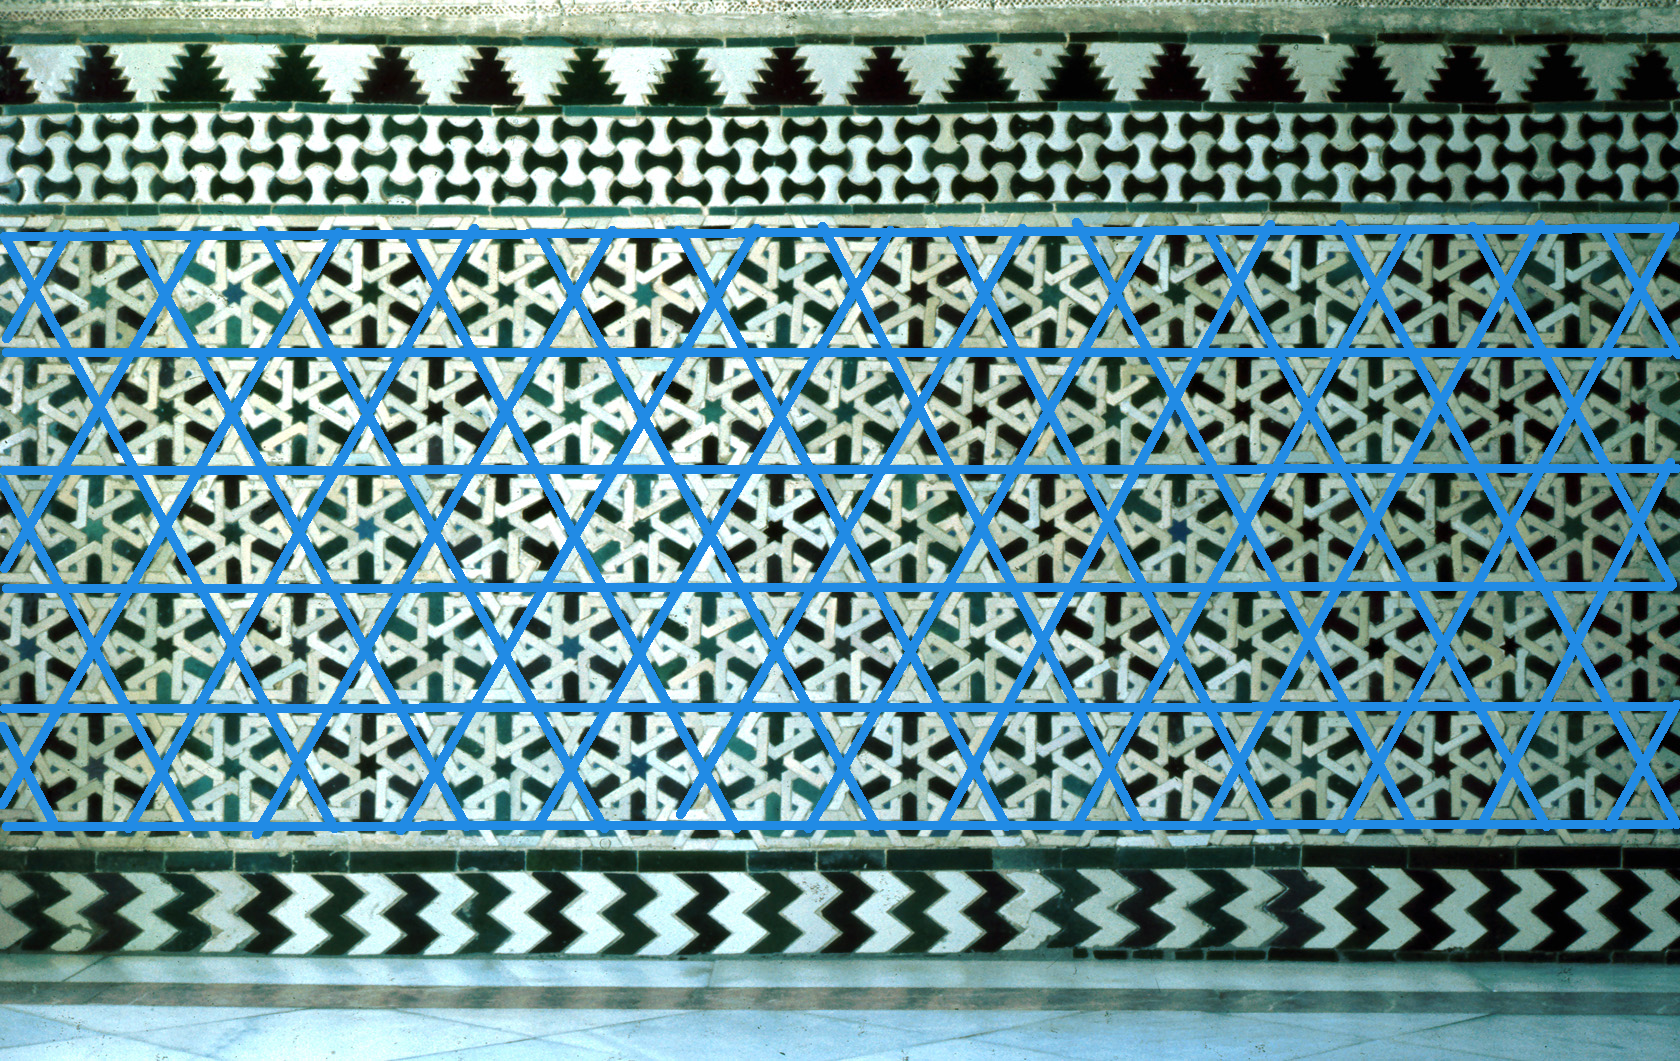
\includegraphics[scale=8]{Alcazar-Kagome.png}}
          \only<3>{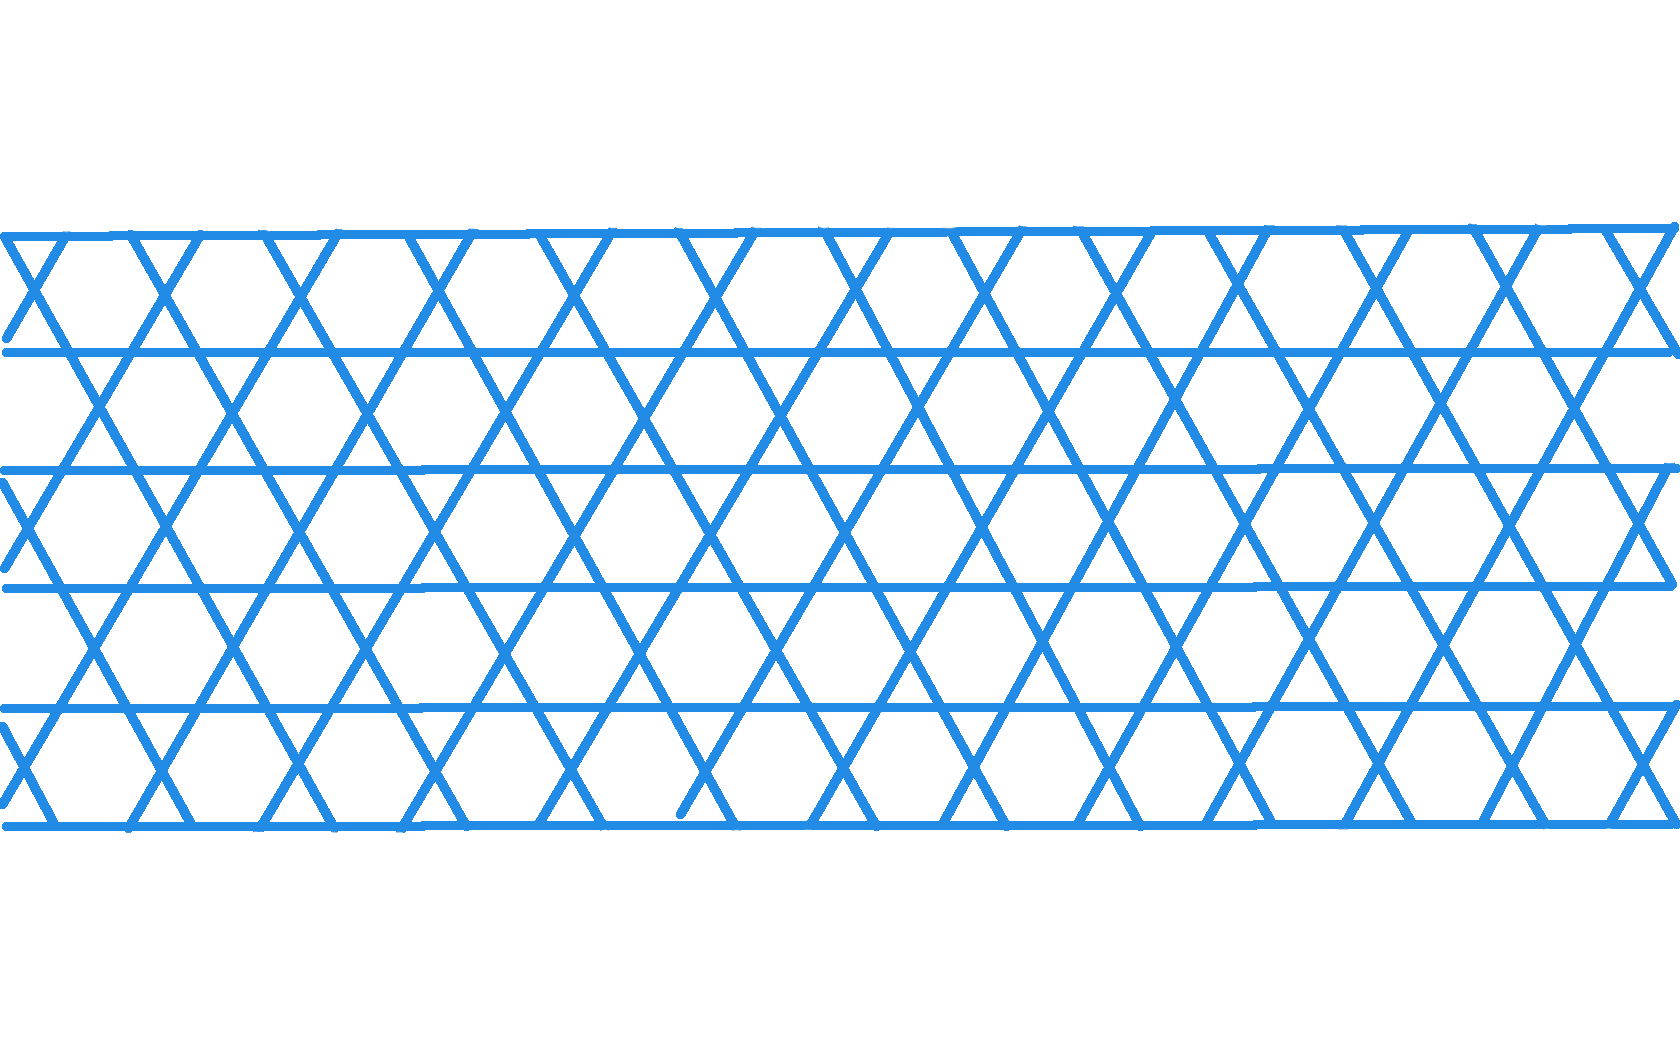
\includegraphics[scale=8]{Kagome.png}}
          % \only<4>{\includegraphics[scale=8]{Spins.png}}
          % \only<5>{includegraphics[scale=8]{HAF.png}}
          
          \uncover<1-2>{\tiny{source: patterninislamicart.com}}
        \end{center}
      \end{frame}

\section{La quantification de Toeplitz}

\subsection{Construction g\'eom\'etrique}


\begin{frame}\frametitle{Quantifications}
\begin{center}
	\begin{tabular}{|c|c|}
		\spline
	    Mécanique classique & Mécanique quantique\\
		\spline
		\uncover<2->{Variété symplectique $M$} & \uncover<2->{Espace de Hilbert $H$}\\ 
		\spline 
		\uncover<3->{Fonction $a\in C^{\infty}(M,\R)$} & \uncover<3->{Opérateur auto-adjoint $A\in L(H)$}\\
		\spline
		\uncover<4->{Flot hamiltonien de $a$} & \uncover<4->{Flot de $e^{itA/\hbar}$}\\
		\spline
	\uncover<5->{Crochet de Poisson} & \uncover<5->{Crochet de Lie}\\
		\spline
	\end{tabular}\end{center}
	\begin{itemize}
	\uncover<6>{\item Quantification : pour un modèle donné de mécanique classique, comment construire un modèle quantique associé ?
	
	\item Semi-classique : le modèle quantique dépend d'un petit paramètre $\hbar$. Que dire de l'asymptotique $\hbar \to 0$ ?}
	\end{itemize}
\end{frame}

\begin{frame}
  \frametitle{Quantification de Weyl et quantification
    g\'eom\'etrique}
  Deux approches historiques diff\'erentes.
  \begin{enumerate}
  \item Ann\'es 30 (motivations physiques):
    \begin{itemize}
    \item vari\'et\'e $M=\R^{2n}$,
    symbole $a(q,p)$.
  
  \item Espace de Hilbert $L^2(\R^n)$.
  \item Op\'erateur associ\'e : on remplace $p$ par $-ih\nabla$.
  \item Exemple : particule massive soumise à un potentiel:
    \[
      |p|^2+V(q)\rightsquigarrow -h^2\Delta+V\]
    \end{itemize}
  \uncover<2>{\item Ann\'ees 60 (motivations math\'ematiques):
    \begin{itemize}
    \item Vari\'et\'e symplectique v\'erifiant
      $[\omega] \in H^2(M,2\pi\Z)$.
    \item Polarisation: distribution lagrangienne $P$
      int\'egrable.
    \item Espace de Hilbert: sections $L^2$ d'un fibr\'e invariantes par $P$.
    \item Exemple : repr\'esentations irr\'eductibles de
      dimension finie d'un groupe de Lie compact.}
    \end{itemize}
    \end{enumerate}
  \end{frame}

  \begin{frame}
    \frametitle{Fibr\'es pr\'equantifiants et vari\'et\'es de K\"ahler}
    \begin{itemize}
    \item Condition d'int\'egrabilit\'e $\Leftrightarrow$ Existence
      d'un fibr\'e en droites complexes $L\to M$ avec une structure
      hermitienne $h$ telle que $curv(h)=\omega$.
    \uncover<2->{\item Vari\'et\'e de K\"ahler (symplectique, complexe et
      riemannienne) : on prend pour polarisation $T_{1,0}M$.}
    \uncover<3->{\item Espace de Hilbert: $H_0(M,L)$. Limite semi-classique : on
      remplace $L$ par $L^{\otimes N}$, de courbure $N\omega$.}
    \uncover<4->{\item Kodaira: si $M$ est compacte, $\dim H_0(M,L^{\otimes N})$ est
      donn\'ee par Riemann-Roch (polyn\^ome en $N$ de degr\'e $\dim_{\C}M$).}
    \end{itemize}
  \end{frame}

\subsection{Op\'erateurs de Toeplitz}


  \begin{frame}
    \frametitle{Quantification de Toeplitz}
    \begin{defn}
      \begin{itemize}
      \item Le projecteur de Szeg\H{o} $S_N$ est le projecteur orthogonal de
      $L^2(M,L^{\otimes N})$ dans $H_0(M,L^{\otimes N})$.
    
    \item Si $a\in C^{\infty}(M,\R)$, l'op\'erateur de Toeplitz
      associ\'e est \[T_N(a)=S_Na:H_0(M,L^{\otimes N})\mapsto
        H_0(M,L^{\otimes N}).\]
      \end{itemize}
    \end{defn}
  \end{frame}

  \begin{frame}
    \frametitle{Exemple: $\C^n$}
    \begin{itemize}
    \item 
    On peut expliciter les espaces de Hardy et le projecteur de
    Szeg\H{o}.
    \[H_0(\C^n,L^{\otimes N})\simeq \left\{f\text{ enti\`ere
        },\, \int_{\C^n}f(z)e^{-N|z|^2}<+\infty\right\}\]

      \[S_N(z,w)=\cfrac{N^n}{\pi^n}\exp\left(-\frac N2|z-w|^2+iN\Im(z\cdot \overline{w})\right)\]
    \uncover<2>{\item Recette de quantification:
      \[
        T_N(z\mapsto
        \overline{z}^{\alpha}z^{\beta})=N^{-\alpha}\partial^{\alpha}z^{\beta}.
        \]}
\end{itemize}
    \end{frame}

    \section{Analyse du noyau de Szeg\H{o}}

\subsection{Op\'erateurs int\'egraux de Fourier}

\begin{frame}
  \frametitle{Th\'eor\`eme de la phase stationnaire}
  On veut \'etudier des int\'egrales de la forme
  \[
    \int e^{iN\phi(x)}a(x)\dd x
  \]
  dans la limite $N\to +\infty$, où $\phi$ et $a$ sont des fonctions lisses.
  \begin{itemize}
  \uncover<2->{\item L\`a o\`u $\nabla \phi$ ne s'annule pas, on peut int\'egrer
    par parties autant qu'on veut, contribution $O(N^{-\infty})$.}
\uncover<3->{\item L\`a o\`u $\phi$ a un point critique de Morse, apr\`es un
    changement de variable, on a un d\'eveloppement asymptotique car
    \[
      \int e^{iN|x|^2}a(x)\dd x\uncover<4>{=N^{-\frac
        d2}\sum_{k=0}^K\frac{N^{-k}}{k!}\Delta^ka(0)+O(N^{-k+1}).}
      \]}
  \end{itemize}
  
\end{frame}

\begin{frame}
  \frametitle{Phases complexes}
  \begin{itemize}
  \item 
  Si $\phi$ est \`a valeurs complexes, l'\'equation $\nabla \phi=0$
  peut ne pas avoir de solutions dans $\R^d$.
\uncover<2->{\item Il faut prolonger $\phi$ et $a$ de manière analytique, ou
  quasianalytique, dans $\C^d$, puis changer de contour
  d'int\'egration.}
\end{itemize}
  \uncover<3>{\'Enonc\'es pr\'ecis beaucoup plus techniques.}
\end{frame}

\begin{frame}
  \frametitle{Op\'erateurs int\'egraux de Fourier}
  \begin{itemize}
      
  \item Op\'erateurs à noyaux:
    \[
      Af(x)=\int A(x,y)f(y)\dd y.
      \]
  \uncover<2->{\item Application de la phase stationnaire: \'etude des op\'erateurs
    \`a noyaux de la forme
    \[
      A(x,y)=\int_{\xi\in E}e^{i\xi\cdot\Phi(x,y)}a(x,\xi,y)\dd \xi.
    \]
}
  \uncover<3>{\item Op\'erateurs diff\'erentiels: $\Phi(x,y)=x-y$, $E=\R^d$,
    et $a$ est un polyn\^ome en $\xi$.}
  \end{itemize}
\end{frame}
\subsection{D\'eveloppement asymptotique du projecteur de Szeg\H{o}}
\begin{frame}
  \frametitle{Expression du projecteur de Szeg\H{o}}
  \begin{thm}[Boutet-Sj\"ostrand, Shiffman-Zelditch]
    Sur une vari\'et\'e K\"ahler compacte, dans les cartes locales, le
    projecteur de Szeg\H{o} $S_N$ correspond au $N$-ième mode de
    Fourier d'un OIF invariant par une action de $\S^1$.
    \[
      S_N(x,y)=e^{N\Phi(x,y)}\sum_{k=0}^KN^{n-k}a_n(x,y)+O(N^{-n-K-1}).
    \]
  \end{thm}
\end{frame}

\begin{frame}
  \frametitle{Cons\'equences}
\begin{itemize}
  \item 
  On a $\Re\Phi(x,y)<0$ si $x<y$ donc $S_N$ d\'ecroît très vite loin
  de la diagonale, comme pour le cas $\C^d$.
\uncover<2>{\item Près de z\'ero on a \[\Phi(x,y)=-\frac 12 |x-y|^2+i\Im(x\cdot
    \overline{y})+O((x,y)^3),\] donc le cas $\C^d$ est un modèle local
  universel dans l'asymptotique $N\to +\infty$.}
  \end{itemize}
  
\end{frame}

\begin{frame}
  \frametitle{Exemples}
  \begin{enumerate}
  \item $\C\mathbb{P}^1$: dans la projection st\'er\'eographique, on a
    \[
      S_N(z,w)=\frac{N}{\pi}\left(\cfrac{1+z\overline{w}}{\sqrt{(1+|z|^2)(1+|w|^2)}}\right)^N.
    \]
    
  \item $\mathbb{H}$: dans le modèle du disque de Poincar\'e, on
    a
    \[
      S_N(z,w)=\frac{N}{\pi}\left(\cfrac{\sqrt{(1-|z|^2)(1-|w|^2)}}{1-z\overline{w}}\right)^N.
    \]
    
  \end{enumerate}
\end{frame}

\section{Localisation des fonctions propres à basse \'energie}

\subsection{\'Etat de l'art}
\begin{frame}
  \frametitle{Localisation}
  \begin{defn}
    Une suite $(u_N)_{N\in \N}$ où chaque $u_N$ est un élément de
    $H_0(M,L^{\otimes N})$ se \emph{localise} sur un fermé $Z\subset
    M$ lorsque, pour tout ouvert $V$ à distance non-nulle de $Z$, on
    a, quand $N\to +\infty$,
    \[
      \int_V |u_N|^2_h\dd Vol=O(N^{-\infty}).
    \]
  \end{defn}
  \begin{ex}
    Pour $x=(m,v)\in L^*$, la forme $e_x^N:u\mapsto
    \langle v^{\otimes N},u(m)\rangle_{L^*,L}$ est continue de $H_0(M,L^{\otimes N})$ dans $\C$. Son dual
    normalisé $\psi_x^N$, état cohérent en $x$, est localisé en $x$.
  \end{ex}
\end{frame}

\begin{frame}
  \frametitle{Localisation près du lieu minimal}
  \begin{prop}
    Soit $h\in C^{\infty}(M)$ et $E\in h(M)$.

    Si $(u_N)$ est une suite de fonctions propres normalis\'ees de
    $T_N(h)$ avec valeur propre $\lambda_N=E+O(N^{-\epsilon})$, alors $(u_N)$ est
    localisée sur $\{h=E\}$.
  \end{prop}
  \begin{preuve}
    Le d\'eveloppement du noyau de Szeg\H{o} donne un calcul
    fonctionnel
    \[
      T_N(f)T_N(g)=T_N(fg)+N^{-1}T_N(C_1(f,g))+N^{-2}T_N(C_2(f,g))+...
    \]
    Où $C_i$ est un opérateur bidifférentiel de degré $2i$.
    On peut donc estimer $\langle u_N,T_N((h-E)^{2n}),u_N\rangle$
  \end{preuve}
\end{frame}

\subsection{Critères sous-principaux}
\begin{frame}
  \frametitle{Valeur caractéristique}
  Si $q$ est une forme quadratique définie positive sur $\R^{2n}$,
  alors il existe une base symplectique $(e_i,f_i)_{1\leq i \leq n}$
  pour laquelle
  \[
    Q\left(\sum x_ie_i+y_if_i\right)=\sum_{i=1}^n \lambda_i(x_i^2+y_i^2).
  \]
  \begin{prop}
    \[\inf\Sp T_N(Q)=N^{-1}\left(\frac {\tr(Q)}{4}+\sum_{i=1}^n\lambda_i\right).\]
  \end{prop}
  On pose $\mu(Q)=\inf\Sp T_1(Q)$.
\end{frame}

\begin{frame}
  \frametitle{Cas d'un symbole à plusieurs puits}
   \begin{minipage}[l]{0.3\linewidth}
     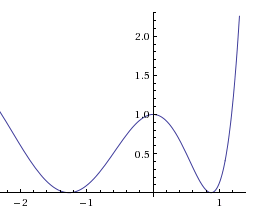
\includegraphics[width=\linewidth]{wells.png}
   \end{minipage}
   \begin{minipage}[r]{0.65\linewidth}
     Que dire si $h$ est minimale en des points critiques non-dégénérés
     ?
     \uncover<2->{
       \begin{thm}[D.]
         Les vecteurs propres de plus petite valeur propre se concentre
         uniquement en les points \og minimaux \fg.
       \end{thm}
     }
     Ce qu'on minimise, c'est le $\mu$ de la hessienne en ce point.
     \end{minipage}
\end{frame}

\begin{frame}
  \frametitle{Cas g\'en\'eral}
  \begin{thm}[D.]
    D\`es qu'il existe $C,\alpha>0$ tel que, pour tout $t\geq 0$, on ait
    \[
      dist(\{h\leq t\},\{h=0\})\leq Ct^{\alpha},
    \]
    alors les vecteurs propres d'énergie plus petite que $\min
    \Sp(T_N(h))+CN^{-\epsilon}$ se concentrent uniquement sur
    \[
      \{h(x)=0, \mu(Hess(h)(x))\text{ est minimal}\}
    \]
  \end{thm}
\end{frame}

\begin{frame}
  \frametitle{Cas particulier 1: Morse-Bott}
  \begin{itemize}
  \item On suppose que $h$ s'annulle à l'ordre $2$ sur une
    sous-variété $Z$ de rang symplectique constant/
  \uncover<2->{\item On a une forme normale locale pour $h$ à symplectomorphisme
    près.}
  \uncover<3->{\item D\'eveloppement asymptotique de la première fonction propre et
    de la valeur propre associé, gap spectral $N^{-\frac 32}$.
  \item Loi de Weyl dans des fenêtres de taille jusque $\epsilon N^{-1}$.}
  \end{itemize}
\end{frame}

\begin{frame}
  \frametitle{Cas particulier 2: Point de croisement}
  \begin{itemize}
  \item $\{h=0\}$ contient un nombre fini de points près duquel il est
    constitué de deux sous-variétés isotropes avec intersection transverse.
  \uncover<2->{\item On a une forme normale locale pour $h$ à symplectomorphisme
    près.}
  \uncover<3->{\item D\'eveloppement asymptotique de la première fonction propre et
    de la valeur propre associé, gap spectral $N^{-\frac 43}$.
  \item Loi de Weyl dans des fenêtres de taille jusque $\epsilon N^{-1}$.}
  \end{itemize}
\end{frame}

\begin{frame}
  \frametitle{Publications}
  Deleporte, A., Low-energy spectrum of Toeplitz operators: the case
  of Wells, Journal of Spectral Theory (accepted).
  \vspace{1em}
  
  Deleporte, A., Low-energy spectrum of Toeplitz operators with a
  miniwell (Arxiv preprint)
  \vspace{1em}
  
  Deleporte, A. Quantum selection for spin systems (preprint).
\end{frame}

\subsection{Perspectives}
\begin{frame}
  \frametitle{Perspectives}
  \begin{enumerate}
  \item Travaux en cours:
    \begin{itemize}
    \item Estimées exponentielles en régularité analytique,
      \uncover<2->{effet tunnel.}
    \uncover<3->{\item Dynamique \`a basse \'energie.}
    \end{itemize}
  \item Conjectures:
    \begin{itemize}
    \uncover<4->{\item O\`u $\mu$ est-elle minimale sur le r\'eseau
      Kagome ?}
    \uncover<5>{\item Le\og Scottish flag\fg{}:
      $T_N(\cos(q)+i\cos(p))$ sur le tore.}
    \end{itemize}
  \end{enumerate}
\end{frame}


\end{document}